\subsection{Recurrent Neural Networks}
\paragraph{Architecture}, let's consider a \emph{computational graph} to compute the
training loss of a recurrent neural network that maps an input sequence of $\bm{L}$ to 
a corresponding sequence of output $\bm{o}$ values. A loss $\bm{L}$ measures how far each
$\bm{o}$ is from the corresponding  training target $\bm{y}$
\begin{figure}[H]
    \begin{center}
        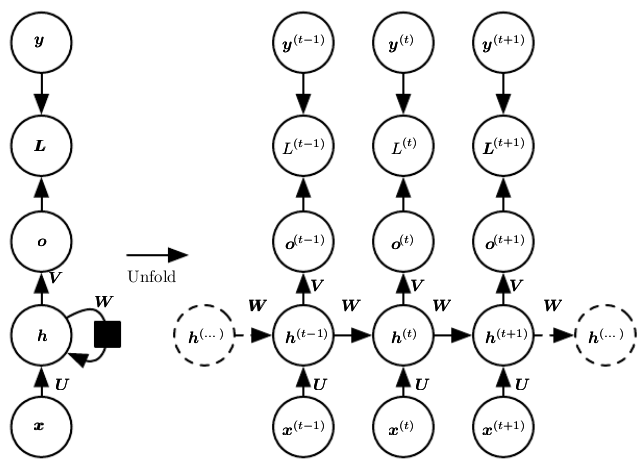
\includegraphics[width=.5\textwidth]{chapters/4_deep_learning/3_types_of_neural_networks/images/03_rnn.png}
    \end{center}
    \caption{Recurrent Neural Networks}
    \label{fig:03_rnn}
\end{figure}


\subsection{Encoder-Decoder Sequence-to-Sequence Architectures}

It is composed of an \uB{encoder RNN that reads} the input sequence and a \uB{decoder
RNN that generates} the output sequence.
\begin{figure}[H]
    \begin{center}
        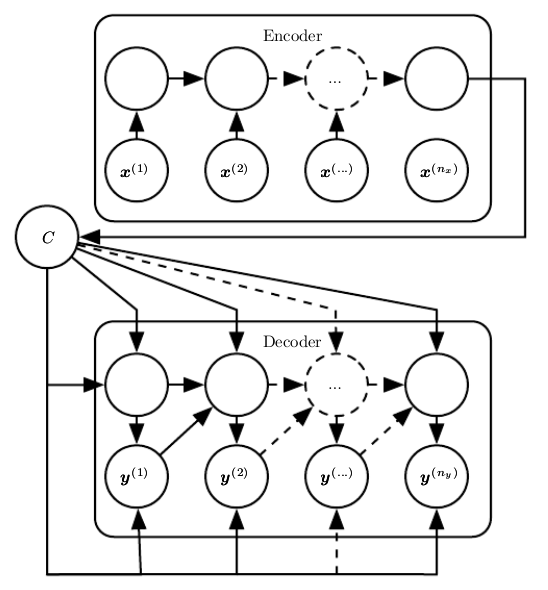
\includegraphics[width=.5\textwidth]{chapters/4_deep_learning/3_types_of_neural_networks/images/03_encoder_decoder_architecture.png}
    \end{center}
    \caption{Encoder-Decoder (or Sequence-to-Sequence RNN) architecture}
    \label{fig:03_encoder_decoder_architecture}
\end{figure}

The \tR{final hidden state of the encoder RNN is used to compute a generally fixed-size
context variable $C$ representing a semantic summary of the input sequence}, then is
given as input to the decoder RNN.

\subsection{The Challenge of Long-Term Dependencies}
\paragraph{The basic problem} is that \uB{gradients propagated over many stages tend to
either vanish or explode}.\\
Consider a very simple recurrent neural network network lacking a nonlinear function:
$\bm{h}_{t} = \bm{W}^{T}\bm{h}_{t-1}$, if we admits an eigen-decomposition of the form
$\bm{W} = \bm{Q}\bm{\Lambda}\bm{Q}^{T}$ with orthogonal $\bm{Q}$ the recurrence may be
simplified further to $\bm{h}_{t} = \bm{Q}^{T}\bm{\Lambda}^{t}\bm{Q}\bm{h}_{0}$.
\uB{The eigenvalues are raised to the power of $t$ causing the eigenvalues with
magnitude lesser than one to decay to zero and eigenvalues with magnitude greater than 
one to explode}.

\subsection{Leaky Units}
\paragraph{Purpose} dealing with long-term dependencies by designing a model operating
at multiple time scales, allowing to \uB{let some parts of the model operating at 
fine-grained time scales to handle small details while other parts operate at coarse
time scales and transfer information from the distant past to the present more 
efficiently}.

\subparagraph{Adding Skip Connections through Time} consists in \uB{adding direct 
connections from variables in the distant past to variables in the present}.\\
By introducing recurrent connections with a time-delay of $d$ to mitigate,
\tB{Gradients now diminish exponentially as a function of $\frac{\tau}{d}$ rather than
$\tau$}

\paragraph{Leaky Units}
Another way to obtain paths on which the product of derivatives is close to one is to
\tB{have units with linear self-connections} and a weight near one on these
connections.
When we accumulate a running average $\mu_{t}$ of some value $v_{t}$ by applying
$\mu_{t} \leftarrow \alpha\mu_{t-1} + (1-\alpha)v_{t}$ the $\alpha$ parameter is an
example of linear self connection from $\mu_{t-1}$ to $\mu_{t}$.\\
\tB{When $\alpha$ is near one, the running average remembers information about the past
for a long time, and when $\alpha$ is near zero, information about the past is 
rapidly discarded}.



\subsection{The Long Short-Term Memory (LSTM) and Gated Recurrent Unit (GRU)}
\paragraph{Purpose}
going further with the idea of self-loops, by making the weight of the self-loop
conditioned on the context rather than fixed.\\
\tB{Self-loops produce paths where the grdient can flow for long duration}.

\begin{figure}[H]
    \begin{center}
        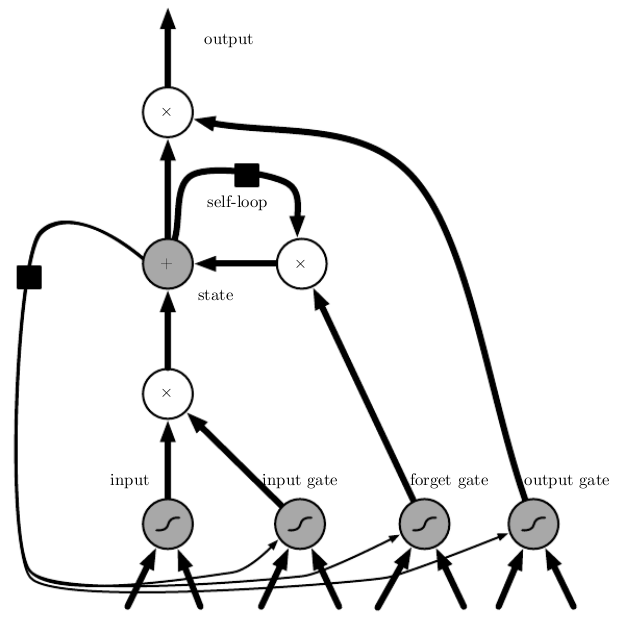
\includegraphics[width=.5\textwidth]{chapters/4_deep_learning/3_types_of_neural_networks/images/04_lstm_rnn_cell.png}
    \end{center}
    \caption{Block diagram of the LSTM recurrent neural network \emph{cell}}
    \label{fig:label}
\end{figure}

Cells are connected recurrently to each other replacing the usual hidden units of
ordinary recurrent networks.

\paragraph{Theory}
The \textbf{forget gate} unit $f_{i}^{(t)}$ for time step $t$ and cell $i$ that sets
the weight to a value between 0 and 1
\begin{center}
    \frB{$f_{i}^{t} = \sigma\left(b_{i}^{f} + \su{j}{}U_{i,j}^{f}x_{j}^{(t)} +
    \su{j}{}W_{i,j}^{f}h_{j}^{(t-1)}\right)$}
\end{center}
with $\bm{x}^{(t)}$ the current input vector, $\bm{h}^{t}$ the current hidden layer vector
containing the outputs of all the LSTM cells, and $\bm{b}^{f},~\bm{U}^{f},~\bm{W}^{f}$ are
respectively biases, input weights and recurrent weights for the forget gates.

